\chapter{Introduction} \label{ch:intro}

%% =====================================================================================
%%
%%              G E N E R A L  I N T R O D U C T I O N
%%
%% =====================================================================================

%% From Just
%A pair of massive stars at the end of their evolution, undergo \ac{SN} explosion, forming, 
%in certain cases, a pair of compact objects orbiting each other. A particular interesting 
%example is a pair of \acp{NS}, compact, but heavy objects sustained against gravitational 
%collapse by the neutron degeneracy pressure. The theory of \ac{GR} predicts that the orbit 
%of the system shrinks, as \acp{NS} loose energy and angular momentum to \acp{GW}. The 
%loss continues until \acp{NS} collide at their last orbit a form an axisymmetric object.
%In this thesis we investigate such a merger, focusing on the aftermath evolution of the 
%remnant. 
%
%The high compactness of \acp{NS} lead to an energetic, explosive merger, where a certain
%fraction of the \ac{NS} matter is ejected from the system at mildly relativistic 
%velocities. In addition to the complex dynamics of the system after merger that might 
%induce additional matter outflows, this makes the \ac{BNS} mergers a strong contributor 
%to the cosmic chemical evolution. The matter ejected at/after mergers, \ie, ejecta, has 
%unique properties, rarely found in other astrophysical cites. Specifically, the abundance 
%of free neutrons allow for the so-called rapid neutron capture process,
%the \rproc{}, that is responsible for the production of the heaviest elements in the 
%Universe, lanthanides and actinides. 
%
%Wide range of possible types and properties of ejecta lead to a similarly broad 
%range in \ac{EM} counterparts to \ac{BNS} mergers. Perhaps, two of the most 
%well studied ones are the \ac{kN}, a thermal counterpart powered by the decay of 
%newly synthesized heavy elements in the ejecta, and \acp{SGRB}, generally non-thermal 
%emission from the ultrarelativistic collimated outflow, formed after the merger. 
%Study of these \ac{EM} counterparts in conjuncture with \acp{GW} emission allows to 
%gain unique insigts into the inner workings of the \ac{BNS} merger and previously 
%unobtainable constraints on the theory of gravity, the properties of matter at 
%supranuclear densities, origin of the \ac{SGRB}, cosmic chemical evolution. 
%
%The complexity, non-linearly, non-stationarity and multidimensionality of physical 
%processes operating at \ac{BNS} mergers on a broad range of scales of length and time 
%implies that self-consistent, quantitative studies are only possible with numerical 
%simulations. These simulations, performed with numerical codes that took years of 
%develop and test, are very computationally expensive, rare and require detailed 
%postprocessing and analysis. Moreover, the self-consistent modeling of the merger and 
%\ac{EM} counterparts is still beyond the reach of modern methods. Generally, the 
%the short-term (hundred of milliseconds) evolution of the merger itself 
%is handled with \ac{NR} codes while the \nuc{} and \ac{EM} emission are evaluated 
%after, in postprocessing. Strengthening the connection between these methods is one of 
%the goals of this thesis. 
%
%In the following sections we sketch the astrophysical background to clarify the 
%context of our study and we conclude the chapter by summarizing the main points of 
%motivation for this thesis and its structural arrangement.


%% <<< From Radice Review >>>
\ac{BNS} mergers are at the center of a variety of physical processes in astrophysics.
The first ever detection of such event by \ac{LIGO}/Virgo \ac{GW} observatories and 
numerous \ac{EM} observatories, \GW{}, have significantly advanced our understanding 
of gravity, physics of dense matter, \acp{SGRB} and origins of \rproc{} elements 
\cite{TheLIGOScientific:2017qsa,Abbott:2018wiz,GBM:2017lvd}. 
%
Emitted during the inspiral, \acp{GW} convey the information about  
constrained \ac{NS} \ac{EOS} at supernuclear densities 
\citep{Hinderer:2009ca,Damour:2012yf,DelPozzo:2013ala}. At even higher, 
densities, several times that of the nuclear mater, the \ac{NS} \ac{EOS} is very 
poorly understood, and the detection of the postmerger \ac{GW} signal, 
emitted by the merger product, the remnant, might shed light on it 
\citep{Sekiguchi:2011mc,Radice:2017lry,Most:2018eaw,Bauswein:2018bma}, 
constraining one of the main quantities, the tidal deformability.
%
The conditions within matter ejected at mergers, ejecta, are sufficient for the \rproc{} 
\nuc{}, responsible for the production of the heaviest elements in the Universe
% such as gold 
\citep{Cowan:2019pkx}.
Whether \acp{BNS} mergers is the prime source of this material is still unknown.
% This was confirmed by \ac{MM} observations of \GW{} \cite{12}. 
% however, it is unclear whether \ac{BNS} mergers is the dominant source of 
% \rproc{} elements in the universe, or if other \rproc{} cites are required to 
% explain the observed abundances in the oldest stars, \ac{UFG} and our solar system. 

Single \acp{NS} are very compact but massive objects, 
%where compactness $C_{i} = GM_i/R_i^2c^2\propto0.15$ and 
for description of which the effects of \ac{GR} cannot be neglected.
A pair of \acp{NS} orbiting each other slowly loses the 
angular momentum to \acp{GW}. The timescale for the radiation reaction, however, 
is much longer than the orbital period for most of the inspiral and the 
system evolution can be considered adiabatic. 
% For instance, the inspiral can be considered as a sequence of circular orbits. 
% However, during last orbits before merger, the finite size (tides) and \ac{HD}
% effects starts to become important. 
The inspiral ends at the onset of the Roche lobe overflow, when the binary 
reaches the mass-shedding limit \citep{Bejger:2004zx}.

In order to study the dynamical phase of \ac{BNS} mergers and \pmerg{} evolution, 
sophisticated \ac{NR} simulations are required. Modern, state-of-the-art methods 
include full \ac{GR}; composition-dependent nuclear \ac{EOS} with finite-temperature 
effects, \ac{GRMHD}; advanced neutrino transport (with varying degree of approximation,
\citep{Sekiguchi:2011zd, Wanajo:2014wha, Foucart:2015gaa, Palenzuela:2015dqa, Sekiguchi:2016bjd, Kiuchi:2017zzg, Radice:2017zta, Fujibayashi:2017puw}.

%In this thesis we perform \ac{NR} simulations of \ac{BNS} mergers, report on their 
%qualitative and quantitative picture and its implication for the \ac{EM} signatures.
%We focus on the nuclear astrophsyics aspect of the mergers, and on the comparison 
%between theoretical predictions and observations of \GW{}, discussing the 
%\rproc{} \nuc{}, thermal \ac{EM} transient, and non-thermal \ac{EM} afterglow. 

In this section we provide a brief summary of the current understanding of the 
\ac{BNS} mergers, their impact on the galactic chemical evolution, and their 
\ac{EM} counterparts. For the sake of brevity we allude most of the technical details, 
and we refer the interested reader to the following reviews and references therein.
%
For the general overview on the topic we refer to \citet{Shibata:2016},
For a more recent reviews done by different leading groups we refer to 
\citet{Radice:2020ddv,Bernuzzi:2020tgt,Shibata:2019wef}.
%
For the discussion on \ac{EM} counterparts to mergers we refer to 
%For the most recent reviews on the topic we recommend the following reviews:
%Radice, for the discussing of the \pmerg{} dynamics and ejecta,
%Bernuzzis, for the \ac{GW} aspect of the mergers \cite{Bernuzzi:2020tgt}
%Shibata \& Hotokezaka for the discussing of the ejecta \cite{Shibata:2019wef}.
\citet{Kumar:2014upa,Fernandez:2015use,Metzger:2019zeh}.

%This chapter is organized as follows...
%First we discuss the observational context of the \ac{BNS} mergers, focusing on the 
%ejecta \nuc{} and \ac{EM} counterparts.
%Then we overview the current picture of \ac{BNS} mergers with emphasis on the 
%\pmerg{} dynamics and mass ejection mechanisms. 
%Finally, we state the goals of this thesis.




%% =====================================================================================
%%
%%              T H E O R E T I C A L  P I C 
%%
%% =====================================================================================

%\section{Theoretical picture of \ac{BNS} mergers}

%In This section we briefly overview the current understanding of the \ac{BNS} 
%merger, the dynamics of the inspiral, effects of tides, \pmerg{} hydrodynamics 
%and open questions.

%% --------------------------------------------------------------------------
%%               I N S P I R A L
%% --------------------------------------------------------------------------

\section{Inspiral}

If \acp{NS} formed through a classical stellar evolution channel of the massive binary, 
their orbit is mostly circular with little to non eccentricity \citep{Aasi:2013wya}. 
%
The binary system looses energy to the emission of \acp{GW}, and the orbit of \acp{NS} 
shrinks. Stars inspiral increasingly fast. The last ${\sim}10^3$ orbits, can be completed in 
a matter of minutes. During the last part of the inspiral, the \ac{GW} signal rises in 
frequency and amplitude (so-called chirp), reaching the peak at the \textit{moment of merger}.

%% ---------------------------
\subsection{Two Body Dynamics}

The dynamics of two stars, that are sufficiently separated to have relatively small 
angular velocity (\ie, quasi-adiabatic inspiral of point-masses) 
the \ac{PN} approximation to \ac{GR}, 
(the expansion in $\upsilon/c$, with $\upsilon/c\ll 1$) is applicable.
%In other words, this is the stage of evolution when the orbital timescale is 
%significantly larger than the orbital one, \ie, $\dot{\Omega}/\omega^2\ll 1$.
%
The amplitude and the phase evolution of the \ac{GW} signal, at the leading order, 
is given by the quadruple formula \citep{Radice:2020ddv} 
%
\begin{equation}
\label{eq:intro:gw_wave}
h(t) \sim \frac{1}{d}\mathcal{M}_c^{5/3} f_{GW}^{2/3} = \nu\frac{M}{d}(Mf_{GW}(t))^{2/3}, \hspace{5mm} 
\phi(t) \sim 2\mathcal{M}_c^{-5/8}t^{5/8} = 2\nu^{-3/8}(t/M)^{5/8},
\end{equation}
%
where $\mathcal{M}_c = M\nu^{3/5}$ is the chirp mass, $M = M_A + M_B$ is the binary mass, 
$\nu = M_A M_B/M^2$ is the symmetric \mr{}, $f_{GW} = \dot{\phi}$, $d$ is the distance of the source.
%Here, the $G=c=1$ are the units, and geometric coefficients are neglected for brevity.
%
Obviously, \acp{NS} are not point-masses. The finite size (tidal) effects modify the 
inspiral and, consequently, emitted \acp{GW}. 
%In the \ac{PN} formalism these effects enter and $5$th \ac{PN} order.
%
%The \ac{PN} expansion, being the asymptomatic expansion, looses its accuracy at high 
%frequencies $f_{GW}\gtrsim 50\,$Hz. 
%
Another approximation to the two-body dynamics in \ac{GR} is the \ac{EOB} formalism,
which is a Hamiltonian formalism, applicable to all stages of the binary evolution.
%It is has an advantage of being applicable both at low and high frequencies and can be 
%applied throughout the inspiral, merger na \pmerg{} \cite{28}.
It is spiritually similar to the way, commonly used in Newtonian dynamics to 
describe the motion of two bodies via the motion of a single body with effective mass 
$\mu=\nu M$ in the effective potential. Approximating the dynamics in \ac{GR} requires 
employing effective particle, $\mu$ and defective metric. 
%
\citet{Damour:2009wj} extended the \ac{EOB} formalism to \ac{BNS} mergers by 
introducing finite size effects. For the up-to-date review we refer tp \cite{Damour:2012mv}.


%% ------------------------------------
\subsection{Effects of tides}

A method to treat the finite-size effects in self-gravitating objects in \ac{PN} 
dynamics was proposed by \citet{Damour:1983a} and is based on ``skeletonizing'' 
objects into worldlines with global properties. This constitute the \textit{outer problem}.
%
It was matched to the \textit{inner problem}, that considered how the worldtube 
around one body is influenced by another. In the case of \ac{BNS}, the latter is 
referred to the tidal effects induced by the external gravitational field of the companion. 
%Matching the outer problem with the inner translates into the inclusion of the tidal 
%deformation effects into the orbital dynamics (and consequently, \ac{GW} emission). 
The fully relativistic formulation of the inner problem was derived in 
\citet{Hinderer:2007mb,Damour:2009vw,Binnington:2009bb}. 
%The key parameters of the formulation are the 
%external tidal moments,
%introduced as symmetric-trace-free projections of the derivatives of the externally 
%generated parts of the local gravitoelectric, $\bar{E}_{\alpha}$ and gravitomagnetic, 
%$\bar{B}_{\alpha}$, fields that read 
%$G_L^A = \partial_{\langle L-1}\bar{E}^A_{\alpha_l\rangle}|_{X^{\alpha}}\rightarrow 0$, 
%(where $X^{\alpha}$ are local coordinates \cite{32}).
%In the local frame of the first body, the \red{internally generated mass} $M_L ^A$ and spin 
%$S_L ^A$ multipole moments, (here $L=i_1,i_2,...,i_l$, is the multi-index) depend on the external
%tidal moments via 
%\textit{tidal polarizability coefficients} $\mu_l$ and $\sigma_l$, expressed as 
%
%\begin{equation}
%    M_{L}^{A} = \mu_l G_{L}^A, \hspace{5mm} S_{L}^A = \sigma_l H_L^A,
%\end{equation}
%
%where $M_L ^A$ and $S_L ^A$ are the internally generated mass and spin miltipole moments.
%(here $L=i_1,i_2,...,i_l$, is the multi-index), and 
%$G_{L}^A$ and $ H_L^A$ are the external tidal moments, related to gravitoelectric and 
%gravitomagnetic fields respectively. 
The key components of the formulation are the external gravitoelectric 
(gravitomagnetic) fields, $l$-th order of which induces the mass (spin) multipolar moments 
of the same order $l$ in \ac{NS}. These moments are characterized by %$G\mu_l$ ($G\sigma_l$), 
tidal polarizability coefficients, that can be written as dimensionless relativistic 
Love numbers \citep{Damour:2009vw,Binnington:2009bb}.
%
%The $l$-th order (external) gravitoelectric (gravitomagnetic) fields induce $l$-th order 
%mass (spin) multipolar moments in a \ac{NS}, characterized by respective coefficients, 
%$G\mu_l$ ($G\sigma_l$), that have dimensions of [length]$^{2l+1}$.
%%
%The dimensionless relativistic Love numbers are defined as
%%
%\begin{equation}
%k_l = \frac{(2l - 1)!!}{2}\frac{G\mu_l}{R^{2l + 1}}, \hspace{5mm} j_l = \frac{(2l-1)!!}{2}\frac{G\sigma_l}{R^{2l+1}},
%\end{equation}
%
%where $R$ is the radius of a \ac{NS}. 
%In many studies, only the dominant $l=2$ mode is considered, \eg, \cite{33}. 
%For \acp{BH}, $\mu_l=\sigma_l=0$ \cite{32,34}.
%Sometimes, only dominant quadrupole $l=2$ gravitoeletric coeffcient is considered \cite{33}.
%
If the external field can be viewed as quasi-static (``adiabatic tides'') the 
Love numbers can be computed by considering the stationary perturbations of the spherical 
relativistic star, \ie, solving the \ac{TOV} equations, which are considered in full \ac{GR}, 
due to strong dependency of the tidal coefficients on the star compactness, defined as 
$C_{i} = GM_i/R_i^2c^2$. 
%
Thus, Love numbers carry the imprint of the \ac{EOS} on the \ac{BNS} dynamics.
%
%On the other hand, if the external field is dynamic, than the effects induced by a \ac{NS}, 
%at linear order in the deformation, can be formulated as a superposition of the proper modes 
%of the \ac{NS}. The excitation of modes occur when the resonant frequency of modes is matched 
%by the star's orbital frequency. 
%This approach has been studied in Newtonian gravity, in \ac{GR} for a test-mass circling the 
%\ac{NS}, and for \acp{NS} of similar mass in \ac{PN} theory \cite{35,36,37}.
%Dynamical external field induces ``dynamical tides'', among which the most important are the 
%pressure modes ($f$-modes) in the non-resonant way\footnote{
%    The resonance for $f$-modes occur in kHz
%    regime, that is achieved only at merger, when two \acp{NN} are no longer isolated objects. 
%    Other mode,s such as $g$- and $r$-modes do not contribute significantly, due to their 
%    lower energies (albeit also lower frequencies).
%}
%
%The tidal effects can be included into the \ac{PN} two-body dynamics by modifying the 
%\ac{GR} effective action as 
%%
%\begin{equation}
%S = S_{GR} + S_{pointmass} = \frac{1}{16\pi G}\int R\sqrt{|g|}dx - \sum_{A}\int M_A \dd s_A
%\end{equation}
%%
%where the last term of the \ac{RHS} is the ``skeletonized'' representation \red{as} a point mass, 
%with non-minimal coupling of worldlines, that read 
%%
%\begin{equation}
%S_{nonminimal} = \sum_{A}\frac{\mu_l^{A}}{2l!}\int (G_L^A)^2 \dd s_A + \frac{l \sigma_l^A}{l! 2(l+1)} \int(H_{L}^A)^2 \dd s_A.
%\end{equation}
%%
%The added term changes the dyanmics at $5$th \ac{PN} order. The change is linear in tidal deformations.
%%
%At the leading \ac{PN} (Newtonian) order, only $l=2$ gravitoelectric terms appear when tidal 
%contributions are included. The term reads 
%%
%\begin{equation}
%\label{eq:intro:tidal_largangian}
%L^{LO}_{tidal} = k_2^A G M_B^2\frac{R_A^5}{r^6} + (A\leftrightarrow B),
%\end{equation}
%%
%where $r$ is the distance between \acp{NS}. 


Writing the modified \ac{GR} action with the inclusion of ``skeletonized'' representation
of a \ac{NS}, the tidal effects can be added into the \ac{PN} description of the two-body dynamics.
The resulted Lagrangian, at the leading (Newtonian), order shows that at small distances 
between stars, $r$, the introduced corrections are attractive. 
%
Further, the Kepler law, given by the quadrupolar gravitoelectric term, 
%
%\begin{eqnarray}
%\Omega^2 r^3 = G M \Big[ 1 + 12 \frac{M_A}{M_B} \frac{R_A^5}{r^5} k_2^A + (A\leftrightarrow B) \Big].
%\end{eqnarray}
%
shows that the finite-size effects manifest as an increased orbital frequency at a given radius.
In other words, the \acp{NS} spin faster if tidal effects are present and merge sooner 
producing signal with higher frequency \citep{Damour:2009wj}. 
%When $r=R_A+R_B$, the frequency at merger can be estimated. 
%There, $2GM\Omega\approxeq2(M_B/(MC_B) + M_B/(MC_B))^{-3/2}$ \cite{29}. 
%For \acp{NS} of the same mass one obtains 
%%
%\begin{equation}
%f_{GW}^{contact} \approxeq 1.327 \Big( \frac{C}{0.15} \Big)^{3/2} \Big( \frac{M}{2.8M_{\odot}} \Big) \text{kHz}.
%\end{equation}
%
%Simulations show that the contact between the two \acp{NS} happens approximately 2-4 \ac{GW} cycles 
%prior to merger at an even lower frequency \cite{38}

Within the \ac{EOB} framework, the dynamics of the system can be expressed in terms of the 
effective Hamiltonian, $H_{EOB}$
%that for zero-spin case can be written 
%%
%\begin{equation}
%H_{EOB} = M\sqrt{1 + 2\nu (\hat{H}_{eff} - 1)}, 
%\hat{H}_{eff} = \frac{H_{eff}}{\mu} = \sqrt{A(u;\nu)(1 + p_{\phi}^2u^2 + 2\nu(4-3\nu)u^2p_{r^*}^4) + p_{r^*}^2}
%\end{equation}
%%
%where $u=GM/rc^2$ is the Newtonian potential. 
%Consder the Schwarszchild spacetime and a particle in it with $\nu\rightarrow0$ and 
%$A(u;0) = 1-2u$. Then, the $H_{eff}$ becomes the particle Hamiltonian.
%
.
The finite-size effects can be included as tidal component of the field potential, $A$, as 
$A = A_0 + A_{tidal}$ \citep{Bini:2012gu}, 
%that can be written as 
%%
%\begin{equation}
%A_{tidal} = \sum_{l\geq 2}\Big[ k_l^{A+}u^{2l+2}(1+\alpha_1^{(l+)}u ... ) + k_{l}^{A-}u^{2l+3}(1+\alpha_1^{(l-1)}u + ...) + (A\leftrightarrow B) \Big]
%\end{equation}
%%
%where $\alpha_i^{(l)}(\nu)$ are coefficients and 
%%
%\begin{equation}
%k_{l}^{A+} = 2k_l^A\big( \frac{M_A}{MC_A} \big)^{2l+1}\frac{M_B}{M_A}, \hspace{5mm} k_l^{A-} = 2j_l^A\Big( \frac{M_A}{M C_A} \Big)^{2l + 1} \frac{M_B}{M_A}
%\end{equation}
%%
%are the multipolar tidal polarizability coupling constants. 
that in turn depends on the multipolar tidal polarizability coupling constants $k_{l}^{A\pm}$.
%
In the Newtonian limit the \ac{EOB} Hamiltonian then reads 
%
\begin{equation}
H_{EOB} \approxeq Mc^2 + \frac{\mu}{2}p^2 + \frac{\mu}{2}(A-1) = Mc^2 + \frac{\mu}{2}p^2 + 
\frac{\mu}{2}\Big( -\frac{2 G M}{c^2 r^2} + \cdots - \frac{\kappa_2^T}{r^5} \Big).
\end{equation}
%
where $\kappa_2^T = \kappa_2^A + \kappa_2^B$ is the constant accounting for the tidal 
interactions at leading order.
%
For a physically motivated range of masses $(1-2)\,\Msun$ and \mr{}s $q\in[1,2]$ the 
$\kappa_2^T\sim[50,500]$. 
%
Similarly, one can defile the $\Lambda_2^i = 2/3 k_2^i (c^2 R_i/GM_i)^5$ with $i\in\{A,B\}$.
Then, instead of $\kappa_2^T$, the \textit{reduced tidal deformability} is used
%
\begin{equation}
\label{eq:intro:Lambda}
\tilde{\Lambda} = \frac{16}{13}\frac{(M_A + 12M_B)M_A^4}{M^5}\Lambda_A + (A\leftrightarrow B).
\end{equation}
%
Consequently, the effects of tides appear in waveform calculations, as radiation reaction 
compliments the conservative dynamics discussed above \citep{Damour:2008gu} 
and discussed in \citet{Damour:2012yf,Banihashemi:2018xfb}.

%At leading order the stationary phase approximation of the waveform reads
%%
%\begin{equation}
%h(f) = Af^{-7/6}e^{-i(\Psi_0(x) + \Psi_{tidal}(x))} = Af^{-7/6}e^{-i(\Psi_0(x)-39/4\kappa_2^Tx^{5/2})}
%\end{equation}
%%
%where $x(f) = (\pi G M f / c^3)^{2/3}$ and $\Psi_0(x)$ is point-mass phase.
%
The $k_2^T$ fully determines the tidal contribution to the waveforms at leading order. 
Hence, from observed \ac{GW} signal, the $k_2^T$ (or $\tilde{\Lambda}$) can be well estimated. 
%
%There have been extensive tests of the \ac{EOB} formalism for \ac{BNS} mergers agains \ac{NR} 
%simulations \cite{43,38,44,45,46}. 
%The accuracy of the \ac{EOB} approximation of tides, the $A_{tidal}$, decreases during 
%the last orbits and for very large $k_2^T$. Modified versions of \ac{EOB} were developed 
%with gravitational self-force calculations of tides computed at high-order TEOBResumS 
%\cite{44,47,46,48} and dynamical tides (SEOBNRT) \cite{49}.
%When spin cannot be neglected, the tidal interactions become more complex \cite{50,51}.
%The oblateness of a spinning \ac{NS} leads to the deformed gravitational field that is 
%characterized by the quadrupole tensor, and produces an attractive contribution to the 
%potential, modifying the inspiral at the $2$nd \ac{PN} order $\mathcal{O}(\upsilon/c)^4$
%\cite{50}. 
%There are also hybrid models of \ac{EOB} and \ac{NR} \cite{52,53}

%% -------------------------------------
\subsection{Gravitational Waves}

The most accurate way to compute waveforms is to conduct \ac{NR} simulations with microphysical 
\ac{EOS}. However, these simulations are computationally expensive and not available or feasible 
for certain areas of the parameter space. The \ac{EOB} approach allows to compute the waveforms 
for the broad range of frequencies and covers all stages of the binary evolution. 
%The \ac{EOB} models can be augmented with the formalism describing the high frequency emission 
%of the remnant (kiloHertz), that itself can be build from the 
%available \ac{NR} \ac{HD} simulations \citep{Bernuzzi:2015rla,Chatziioannou:2017ixj,Easter:2018pqy}.

The \ac{GW} signal observed with ground-based facilities, contains information 
about the chirp mass, 
%(related to $I_{-10}$),
%where $I_p = \int \dd\ln f(\gamma(f))f x^{2p}(f)$ with $\gamma(f)df$ being the 
%measure of the detector noise \cite{59,6},
primarily at low frequencies. Additionally, the low frequency part of the signal, 
${\leq}50\,$Hz and ${\leq}100\,$Hz, contains information on the symmetric \mr{} and \ac{SNR}.
On the other hand, the information about tidal effects (tidal parameters) is related to 
%$I_{+10}$,
higher frequency signal, evaluation of which requires accurate high-frequency waveforms.


From the Newtonian limit discussed above, it follows that the system dynamics at merger 
is determined mainly by $\kappa_2^T$ \citep{Bernuzzi:2014owa}. \ac{NR} simulations verified this 
prediction \citep{Zappa:2017xba,Breschi:2019srl}. 


With respect to the \GW{} most of the information was obtained in $30-600$~Hz frequency 
range (${\sim}1300$ orbits).
The signal was interpreted as coming from the \ac{BNS} merger with total mass of ${\simeq}2.7\,\Msun$,
chirp mass $\mathcal{M}=1.186(1)\,\Msun$, \mr{} $q\in[1,1.34]$ and $\tilde{\Lambda}{\simeq}300$ 
(with an upper bound of ${\sim}800$) \citep{TheLIGOScientific:2017qsa,Abbott:2018wiz,LIGOScientific:2018mvr}.
Inclusion of the \ac{EM} counterparts into the analysis resulted in higher $\tilde{\Lambda}$ being 
more favored \citep{Radice:2017lry,Radice:2018ozg,Breschi:2021tbm}.
%
The estimation of individual masses and \mr{} was more uncertain and depended on the 
prior chose for the spin \citep{Abbott:2018wiz}. Due to the partial degeneracy between tidal 
parameters and the \mr{}, the \ac{EOS} constraints are also subjected to uncertainties. 
%Specifically, assuming that stars had small spin ${\leq}0.05$, the stars radii can be 
%constrained to $11-12$~km \cite{De:2018uhw,Abbott:2018exr}. 
%Assuming also that \ac{EOS} can support a non-rotating \ac{NS} with a mass $1.97\Msun$, 
%results in  $R\sim 11.9\pm 1.4$~km and $90\%$ credibility \cite{Abbott:2018exr}.
%
%\ac{GW} signal during the inspiral (including tidal phasing) also provides constraints 
%on the \ac{EOS} viewed in the pressure-density diagram \cite{65}. 
%For an example case of a \ac{BNS} with $\rho_{\rm max} \approxeq 2 \rho_0$, 
%the estimated value of pressure is $P(2\rho_0)=3.5_{-1.7}^{2.7}\times10^{34}$ dyn cm$^{-2}$ 
%at $90\%$ confidence level.
%
%For \GW{} the peak of the \ac{GW} signal, the merger, was not detected. However, from the 
%probability distribution of $\tilde{\Lambda}$, adopting \ac{NR}-motivated fitting 
%formula, it is possible to asses the peak frequency that falls in $1.2 - 2$kHz \cite{55}.
%The \ac{GW} peak luminocity is estimated to be $\geq 0.1\times 10^{56}$ erg/s \cite{61}. 


%% --------------------------------------------------------------------------
%%               P O S T - M E R G E R
%% --------------------------------------------------------------------------

\begin{figure}[t]
    \centering
    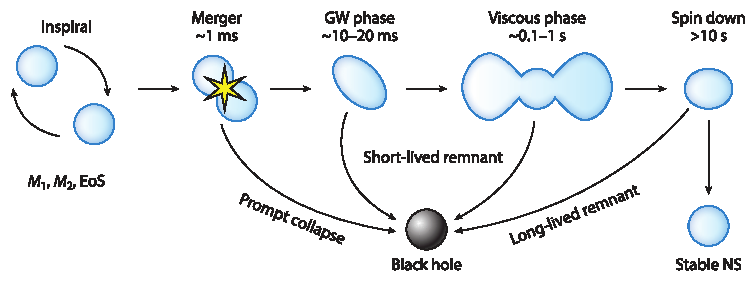
\includegraphics[width=0.70\textwidth]{Fig_3_Rad.pdf}
    \caption{
        Overview of the different phases in an \ac{NS} merger and the relative timescales. 
        The inspiral ends with the merger, when the two stars start to fuse together. 
        The early \pmerg{} evolution is entirely driven by hydrodynamics and by \ac{GW} emission. 
        If the remnant does not collapse within ${\sim}10-20\,$ms, \ac{GW} losses
        subside and other physical processes become more important: 
        Angular momentum redistribution (which is due to turbulent viscosity) 
        and neutrino losses operate over a timescale of a tenth of a second to a few
        seconds. This is also the characteristic timescale for the evolution of the remnant disk. 
        If the remnant does not collapse over a timescale of a few seconds, then it will 
        spin down because of \ac{MHD} effects over a possibly much longer timescale 
        of several seconds to a few hours. 
        (Adapted from \citet{Radice:2020ddv}).
    }
    \label{fig:intro:RadFig1}
\end{figure}


%% -----------------------------------
\section{Merger and \pmerg{}}
%% ------------------------------------

After the \acp{NS} inspiral and merge, the dynamics of the system becomes significantly 
more complex, as temperatures and densities rise by orders of magnitude and new 
physical effects, \eg, magnetic fields and weak interaction, start to influence the evolution. 
The \pmerg{} phase is not well understood and mainly explored with miltiphsyics \ac{NR} 
simulations with various degrees of sophistication and resolution. 

The summary of the \ac{BNS} \pmerg{} evolution is shown in Fig.~\ref{fig:intro:RadFig1}. 
There are several trajectories that system can take, depending when/if the formed remnant 
collapses to a \ac{BH}. The early \pmerg{} phase is charaterized by strong \ac{GW} 
emission and hydrodynamic effects. After it, several interlinked processes govern the 
evolution, \eg, \ac{MHD} stresses, that contribute to the angular momentum and redistribution, 
and neutrino emission, that alters the matter composition and cools is.
If \ac{BH} does not form, the \ac{MHD} torques and residual \ac{GW} emission spin down 
the remnant.

%% ------------------------------------------------
\subsection{Dynamics and Thermodynamics Conditions}

Prior to the merger, the \ac{NS} can be considered as being in the cold, neutrino-less, 
weak equilibrium with only marginal heating due to tidal deformation at the last orbits.
The dynamics at merger is dominated by the \acp{NS} orbital motion
as $\upsilon_{rad}\ll\upsilon_{orb}$, 
%\footnote{
%    The orbital speed can be written as $\upsilon_{orb}\eqsim\Omega r\eqsim\sqrt{GM/(R_A + R_B)}$
%    that for equal mass binary is $\upsilon_{orb}/c\eqsim\sqrt{C}\eqsim0.39(C/0.15)^{1/2}$.
%    The radial velocity is beven by the evolution of the orbital frequency, as 
%    $\omega_r \eqsim 2\Omega r \dot{\Omega}/(3\Omega^2)$. The $\dot{\Omega}$ can be 
%    estimated from the fact, that orbital frequency satisfies 
%    $\dot{\Omega}_{GW}\sim(3456/125)(G\mathcal{M}/c^3)^5\Omega_{GW}^{11}$ during the 
%    inspiral. Then, the radial velocity reads 
%    \begin{equation}
%    \upsilon_r/c\eqsim\frac{192\pi}{15}\frac{G^3 M^3}{c^5(R_A + R_B)^3}\frac{q}{(1+q)^2}
%    \end{equation}
%    that for equal mass gives $\upsilon_r/c \eqsim 0.0034 (C/0.15)^3$.
%}.
%Merger time, $t_{merg}$, estimated from the \ac{GW} frequency at \acp{NS} collisition 
%for comparable \ac{NS} masses is given by 
%\begin{equation}
%    t_{merg}\eqsim\frac{1}{2f_{GW}^{contact}}\eqsim1.50\text{ms}\Big(\frac{M}{2.8\,\Msun}\Big)^{1}
%\end{equation}
%where the frequency of \acp{GW} when \acp{NS} come into contact, \ie, when the distance 
%between them, $r = R_A + R_B$ can be evaluated from the Kepler law, given by 
%the quadrupolar gravitoelectric term, % Eq.~7
%$2GM\Omega \eqsim 2(M_B/(MC_B) + M_B/(MC_B))^{-3/2}$ \cite{29},
%as 
%\begin{equation}
%    f_{GW}^{contact} \eqsim 1.327 \Big(\frac{C}{0.15}\Big)^{3/2}\Big( \frac{M}{2.8\,\Msun} \Big) \text{ kHz}
%\end{equation}
that is $\upsilon_{orb}\eqsim\Omega r\eqsim\sqrt{GM/(R_A + R_B)}$, indicating that 
more compact binaries experience more rapid, more violent mergers.

%%%% Remnant
%When \acp{NS} collide, their deformed cores squeeze past each other, triggering \ac{KHI},
%in the first bounce. After several of these bounces, the cores fuse into a single object.
At collision, \ac{KHI} is triggered by the \acp{NS} cores plunging into the companion,
squeezing past each other inducing first wave of gravity-driven compression. 
The maximum values of temperatures and densities are reached than \citep{Perego:2019adq}. 
As nuclear and centrifugal forces start to dominate, the cores bounce back until gravity 
takes over again. 
%
Notably, formed in the violent, fast collision, the remnant core while is being far from 
hydrodynamic equilibrium, does not exhibit shocks. This is due to high speed of sound 
of nuclear matter at supra-nuclear densities 
%($c_s\gtrsim0.2\, c$, at $\rho\gtrsim\rho_0$)
.
Shocks, however, form at the \ac{NS} surface, accelerating matter to mildly-relativistic 
velocities %(\ref{Sec:intro:bns:ejecta}).
The fluid inside the cores thus remains cold 
%$T\lesssim10\,$MeV, $s\lesssim1\,k_B$/baryon 
throughout the merger, while at the interface between cores, the compression and shear 
dissipation raises the temperature to $T{\sim}70-110\,$MeV, 
as structure described by a pair of hot regions, offset by $\sim\pi/2$ with 
respect to dense cold regions forms \citep{Kastaun:2016yaf}.
%
Overall evolution proceeds towards more axisymmetric, stable remnant, but can be 
interrupted by the \ac{BH} formation. 

%%%% Disk Foramtion
The matter outside the bouncing cores, lifted by tidal torques and squeezed out at the 
collisional interface, forms a disk (or a torus).
Due to various contributions with different properties, the disk is highly non-uniform.
The overall properties of the disk such as mass, have complex dependency on 
binary parameters, that can be expressed, at a first approximation, via fitting 
formulae to \ac{NR} simulations \citep{Radice:2017lry,Radice:2018xqa,Radice:2018ozg}. 
The generic disk evolution around the remnant consists of quasi-adiabatically expansion
of its outer layers 
%with $T^3/\rho^3\sim\text{const}$ as the \ac{EOS} is dominated by non-relativisitc baryons
and cooling of the inner regions. 
%
As was mentioned above, the newly born remnant is not hydrodynamically stable. 
Its dynamics is characterized by the pronounced $m=2$ bar- and $m=1$ one-armed-
deformations, \red{Refs}, inducing spiral waves, propagating through the 
disk \red{FIG}. Additionally, the former leads to the strong \ac{GW} emission 
in ${\sim}10-20$~ms \pmerg{}. The backreaction from the energy and angular momentum 
loss dumps the $m=2$ mode efficiently and \ac{GW} emission subsides. 
%We refer to this evolutionary phase as \ac{GW}-dominated \pmerg{} phase.
%Notably, the $m=1$ mode, however, can persist due to mode coupling 
%\cite{Dietrich:2016phd}. 
That marks the end of the ``\ac{GW}-driven phase'' of \pmerg{} evolution. 

%%%% Disk Settling down 
Weak processes and spiral density waves, cooling and shocking periodically the 
fluid respectively, bring the disk to the configuration, that can be described by smooth 
temperature profile 
%from $\sim10\,$MeV at $\rho\eqsim10^{13}$\gcm to $\sim0.1\,$MeV at $\rho\eqsim10^4$\gcm
%with entropy $\in(3,10)$ $k_B$/baryon
and quasi-Keplerian orbit.
%
%%%% IF BH forms
If the remnant collapses to a \ac{BH}, the densest part of the disk is 
accreted on the dynamical timescale, reducing the total mass by half 
%and the disk maxiumum density to $\sim10^{12}\,$\gcm,
and disk shrinks \citep{Perego:2019adq}.

%%%% Magnetic fields
While \acp{MF} are not expected to affect the \ac{BNS} inspiral, their influence 
on the postmerger evolution can be strong \citep{Duez:2006qe,Kiuchi:2017zzg}, as they get amplified 
to the values exceeding that of a magnetar, 
%$10^{16}\,$Gauss, 
by a variety of processes, 
\eg, flux freezing and compression, \ac{KHI} at the collisional interface \citep{Kiuchi:2015sga},
\ac{MRI}, \citep{Duez:2006qe,Kiuchi:2017zzg} and \ac{MF} winding \citep{Duez:2006qe},

Whether the ordered, large-scale \acp{MF} can form in \pmerg{} environment 
via the dynamo process is presently unknown. They are important in producing 
polar collimated outflows, jets \citep{Bucciantini:2011kx,Ruiz:2016rai} and mildly relativistic 
outflows \citep{Metzger:2018qfl,Fernandez:2018kax}. Random magnetic fields are also 
relevant for \pmerg{} evolution, as they generate stresses, enhancing angular momentum transport. 
Presently, these processes are not well understood, as seed \ac{MHD} instabilities operate at 
small scales (centimeters) and cannot be resolved in global \ac{MHD} \ac{BNS} merger 
simulations
% with reslistic initial condiitons
.
To be able to resolve the instabilities (to increase their scale), the seed \acp{MF} are 
artificially enhanced to the magnetar-strength \citep{Kiuchi:2015sga,Kiuchi:2017zzg}.
%
%%%% Alpha-viscosity model
The effect of \acp{MF} on the angular momentum transport can be approximated via 
the $\alpha$-viscosity model \citep{Shakura:1972te}. \red{More on it? For the theiry and GRLESS model?}
These effects are important 
in determining the remnant structure, lifetime and hence, the \pmerg{} \acp{GW} 
\citep{Radice:2017zta,Shibata:2017xht}. 
%The timescale for the angular momentum redistribution in the remnant \cite{80} 
%\begin{equation}
%    t_{rem} \eqsim \alpha^{-1}R_{rem}^2\Omega_{rem}c_s^{-2}\eqsim 0.56\,s\Big(\frac{\alpha}{0.001}\Big)^{-1}\Big(\frac{R_{rem}}{15\,\text{km}}\Big)^2 \Big( \frac{\Omega_{rem}}{10^4\,\text{kHz}} \Big) \Big(\frac{c_s}{0.2\,c}\Big)^{-2}
%\end{equation}
%where $\Omega_{rem}$ and $c_s$ are the angular momentum and sound speed respectively.
an the loss of angular momentum brings the remnant closer to either stable, 
rigidly rotating configuration or collapse \citep{Hotokezaka:2013iia}. 
%
The \acp{MF} effects within the Keplerian disk facilitate accretion 
\citep{Fernandez:2015use,Fujibayashi:2017puw,Fernandez:2018kax,Miller:2019dpt},
%on a timescale
%\begin{equation}
%    t_{disk} = \alpha^{-1}\Big(\frac{H}{R}\Big)^{-2}\Omega^{-1}_K \eqsim 0.78 \Big(\frac{\alpha}{0.02}\Big)^{-1}\Big(\frac{H/R}{1/3}\Big)^{-2}\Big(\frac{M_{rem}}{2.5\,\Msun}\Big)^{-1/2}\Big(\frac{R_{disk}}{100\,\text{km}}\Big)^{3/2}
%\end{equation}
%where $M_{rem}$ is the mass of the central remnant and $R_{disk}$ is the radial 
%scale of the disk.

%%%% Neutrinos
The prime cooling mechanism of the post-\ac{GW}-dominated phase is the emission of 
neutrinos, produced in the hot, dense part of the disk and remnant, and that are 
able to escape \citep{Eichler:1989ve,Rosswog:2003rv,Sekiguchi:2011zd}. 
%The typical neutrino mean free path is 
%\begin{equation}
%    \lambda_{\nu} = \Big(n_B\sigma_0(E_{\nu}/m_e c^2)^2\Big)^{-1}\simeq 24.6\,\text{m}\,(\rho/10^{14}\,\text{g}\,\text{cm}^{-3})^{-1}(E_{\nu}/10\,\text{MeV})^{-2},
%\end{equation}
%where $n_B$ is the density of baryons, and 
%\begin{equation}
%    \sigma_0 \simeq 4G_{F}^2 (m_e c^2)^2 / (\pi(\hbar c)^4)\simeq 1.76\times 10^{-44} \, \text{cm}^2
%\end{equation}
%is the typical neutrino cross section scale, and $E_{\nu}$ is the neutrino energy.
%Considering the charactersitic remnant temperature as  $T_{rem}\simeq20\,$MeV 
%energy of the thermal neutrinos then $E_{\nu}\simeq 3.15T_{rem}$ and optical depth 
%$\tau_{\nu}\simeq R_{rem}/\lambda_{\nu}=\mathcal{O}(10^{4})$.
The neutrinos are radiated on a diffusion timescale \citep{Perego:2014fma}.
%\begin{equation}
%    t_{diff} \simeq \frac{\tau_{\nu}R_{rem}}{c}\simeq 4.28\,s\Big( \frac{R_{rem}}{15\,\text{km}} \Big)^{-1}\Big(\frac{M_{rem}}{2.5\,\Msun}\Big)\Big(\frac{T_{rem}}{20\,\text{MeV}}\Big)^2.
%\end{equation}

%%%% neutrinos in the remnant and disk
Within the remnant, neutrinos are in a weak and thermal equilibrium with matter 
due to charged current reactions. There, the production of electron neutrinos, $\nu_e$,
is suppressed by degeneracy and as chemical potential $\mu_n-\mu_p+\mu_e<0$ at high temperatures, 
the electron anti-neutrinos, $\bar{\nu}_{e}$, dominate. The effect of these ``trapped'' 
neutrinos on the remnant evolution is not very strong \citep{Foucart:2015gaa,Perego:2019adq}.
%
Within the disk, however, the optical depth for neutrinos is ${\simeq}1$ so 
the they can diffuse out on a timescale of milliseconds, lowering the disk 
temperature. The cooling rate is controlled by the degeneracy state of neutrinos 
%that is kept at mild values by the feedback negative effect, higher 
%values have on the cooling rate.
\citep{Beloborodov:2008nx}.

During the early \pmerg{}, the luminosity of the electron antineutrinos 
$L_{\bar{\nu}_e}{\gtrsim}L_{\nu_e}$, as the 
free neutrinos are abundant in the disk and the absorption opacity for $\nu_e$ 
exceeds that of $\bar{\nu}_e$.
Thus, alongside heating and decompression, the initially cold matter in weak 
equilibrium, undergoes \textit{leptonization} 
%The heavy neutrinos, $\nu_{\mu,\tau}$, are balanced by pair processes and 
%decouple from matter at higher densities and temperatures within the remnant
%namely $\rho\gtrsim10^{13}$\gcm and $T\gtrsim8\,$MeV 
\citep{Perego:2014fma,Endrizzi:2019trv},
%The, BNS simulations including
%neutrino transport predict the mean neutrino energies at infinity
%$E_{\nu_{e}}(\sim 10\,\text{MeV})\lesssim E_{\bar{\nu}_e}(\sim 15\,\text{MeV}) \lesssim E_{\nu_{\mu,\tau}}(\sim 20\,\text{MeV})$. Notably, binaries with higher mass 
%show higher neutrino energies \cite{14,86}.
\ie, $n+\nu_e\rightarrow p + e^-$. \red{check that, from Wiki}
%
Neutrinos with different energies decouple from matter in different regions.
%due to the stron dependency of the cross section on the incoming neutrino energy.
Mildly energetic $\nu_{e}$ and $\bar{\nu}_e$ decouple at ${\sim}10^{11}\,$\gcm, found 
in the disk, while low energy neutrinos decouple at higher $\rho\sim10^{13}\,$\gcm.
The geometric surface along which neutrinos decouple is usually called ``neutrino 
surface'' \citep{Perego:2014fma,Endrizzi:2019trv}.
%The dependency of the location and the geometry of this surface on the thermodynamics 
%conditions and neutrino energy facilitates the need to coherent treatment of the 
%strong and weak interactions over a broad span of densities and temepratures.
The energy dependent (spectral) neutrino radiation trasport is required in 
\ac{BNS} merger simulations

%%%% Neutrino oscillations
While it has been shown that neutrino flavor conversions may occur in the \ac{BNS} 
\pmerg{} environment, \eg, the matter-neutrino oscillations, induced by the 
the fact that $\bar{\nu}_e$ decouple at smaller radii then $\nu_{e}$ 
\citep[\eg][]{Zhu:2016mwa,Tian:2017xbr}, and fast-flavor conversions above the 
neutrino surface \citep{Wu:2017drk}, their impact on the properties of the ejected 
material remains largely unexplored.
%More works of neutrino quantum kinetics equations \cite{90,91}, that include 
%collisional integral and angular and energy distributions of neutrinos are required.

%%%% EOS 
One of the main unknowns with respect to \ac{BNS} mergers, is the high density part, 
$\rho{\gtrsim}\rho_0$ of the \ac{NS} \ac{EOS} \citep[\eg][]{Hebeler:2013nza,Oertel:2016bki}, that relate to the 
relevant thermodynamic degrees of freedom and nucleonic interactions. For instance, 
the emergence of the new species, \eg, hyperons, pions, muons, and nuclear 
resonances, would lower the matter degeneracy, and thus, soften the \ac{EOS} \citep[\eg][]{Fore:2019wib,Vidana:2010ip}.
Additionally, the emergence of to deconfined quark matter, due to \ac{QCD} phase transition,
would alter \ac{EOS} at very high temperatures and densities that not well constrained 
\cite{Busza:2018rrf}.

%% ---------------------------------------
\subsection{Fate of the Remnant}

The end product of \ac{BNS} merger depends primarily on the binary parameters, (masses, 
\mr{}) and \ac{EOS}, and in particular, on the maximum supported mass of a non-rotating 
\ac{NS}, $M_{max}^{TOV}$ \citep{Shibata:2016}, as well as on the finite temperature and 
non-beta-equilibrium composition effects. 
%
The \ac{BH} formation directly at merger is usually referred to as \ac{PC}. 
The conditions for it depend on \ac{EOS} and are not well understood. 
Simulations show that in equal mass binaries, \ac{PC} occurs if the total mass 
$M\gtrsim M_{thr} = k_{thr}M_{max}^{TOV}$, where $k_thr\in(1.3,1.7)$ that depends on 
\ac{EOS} \citep{Shibata:2005ss,Shibata:2006nm,Hotokezaka:2011dh,Bauswein:2013jpa}.
%(or $\kappa_2^T\lesssim43-73$, or $\tilde{\Lambda}\lesssim338-386$.
Simulations of unequal mass binaries show that the threshold is lower \citep{Bauswein:2017vtn}, 
and $k_{thr}{\propto}C_{1.6}$, with $C_{1.6}$ being the compactness of the $1.6\,\Msun$ 
\ac{NS} \citep{Hotokezaka:2011dh,Bauswein:2013jpa,Bauswein:2017vtn}. 
%As \ac{PC} cases are 
%not expected to ejecta large amount of material and be \ac{EM}-loud (in case of 
%comparable mass binary), the \GW{} is believed to be not a \ac{PC} case, 
%\cite{Margalit:2017dij,Bauswein:2017vtn}. 
%
The remnant that does not undergo \ac{PC} is a massive \ac{NS}, temporarily supported 
by fast rotation \citep{Baumgarte:1999cq,Rosswog:2001fh,Shibata:2005ss,Shibata:2006nm,
    Sekiguchi:2011zd,Hotokezaka:2013iia,Bernuzzi:2015opx}, whose lifetime depends 
intricately on the \ac{EOS}, finite temperature effects, and viscosity. A commonly 
adopted classification, based on the properties of equilibrium models (neglecting the 
dynamical, finite temperature, and magnetic effects), \ie, $M_{max}^{TOV}$ and
$M_{max}^{RNS}$\footnote{
    $M_{max}^{RNS}$ is the maximum mass of a rigidly rotating \ac{NS} (no differential 
    rotation) supported by zero-temperature (cold) \ac{EOS}. Also sometimes referred as 
    mass-shedding limit.
    % $M_{max}^{TOV}$ and $M_{max}^{RNS}$ are agnostic to thermal or magnetic eects 
    %which can impact the stability of the remnant in nontrivial ways (108, 72)
}
distinguishes between 
\ac{HMNS} if $M{>}M_{max}^{RNS}$, 
\ac{SMNS} if $M_{max}^{TOV} {\leq} M_{max}^{RNS}$,
and stable \ac{MNS} if $M {<} M_{max}^{TOV}$ \citep[\eg][]{Baumgarte:1999cq}.
A \ac{HMNS} is supported by differential rotation that viscosity reduces with time. 
Hence, it is expected to collapse to a \ac{BH}. A \ac{SMNS} can avoid the collapse 
even after reaching rigidly rotating configuration. The lifetime of a \ac{HMNS} and 
a \ac{SMNS} depends on the efficiency of mass and angular momentum loss 
(to, \eg, \acp{GW} and massive winds) and finite temperature effects \citep{Radice:2018xqa}. 
%
Discussing the \ac{NR} simulations we shall distinguish between \textit{short-lived} remnants, 
that collapse to \ac{BH} during \ac{GW}-dominated phase, 
% taht correspods to ${\sim}10-20\,$ms after merger \cite{107,60}
and \textit{long-lived} otherwise.

If a remnant can achieve rigid rotation, its evolution then is characterized by the emission 
of \acp{GW} (due to residual asphericity) and magnetic braking, reducing further its 
angular momentum, until either a \ac{BH} forms, or a stable non-rotating equilibrium is reached.
The observations of \acp{SGRB} with X-ray plateu 
\citep{Zhang:2000wx,Lasky:2015lej,Fan:2013cra}, if indeed given by the 
magnetar activity\footnote{
    There are other possible explanations behind the X-ray plateu emission of \acp{SGRB} 
    \citep{Oganesyan:2019jij}
}, suggest that the remnant may survive from seconds to hours \citep{Fan:2013cra,Ravi:2014gxa}.
Most of the energy, ${\sim}10^{52}\,$erg, that a remnant needs to lose before collapsing 
most likely is carried away in form of \acp{GW}, as \ac{EM} observations of \GW{} suggest.
%This emission can be observed for the nearby event \cite{111}, priding direct information 
%on the remnant fate. However this emission was not observed for \GW{} \cite{67,68}

From \ac{EM} observations of the merger the fate of the remnant, albeit in the 
model-dependent way can be inferred. In case of \GW{}, the presence of such counterpart 
strongly disfavors \ac{PC} (as those are not expected to eject any significant amount 
of matter) \citep{Margalit:2017dij,Bauswein:2017vtn,Radice:2017lry}, while leaving 
the question whether it was \ac{HMNS} or \ac{SMNS} open. \citet{Margalit:2017dij} suggested 
that the remnant was short-lived, on account of the non-detection of the expected ${\sim}10^{52}\,$erg, 
from the spin-down of the long-lived one. Assuming thus that \GW{} produced a \ac{HMNS}, 
allows to put a constraint $M_{max}^{TOV}{\lesssim}2.2\Msun$ \citep{Margalit:2017dij}.
%
On the other hand, if the magnetar model of \acp{SGRB} is applied to \GW{} 
\citep{Ai:2018jtv,Li:2018hzy,Piro:2018bpl}, the remnant is required to be long-lived
(months) and exhibit weak dipol \acp{MF} \citep{Ai:2018jtv}, leading to a different 
constraint on the maximum mass of the non-rotating star, $M_{max}^{TOV}{\gtrsim}2.2\Msun$ 
%and up to an order of magnitude lower ejecta mass ${\sim}10^{-3}\,\Msun$, that is attributed 
%to reducied amount of emergy from radioactive decay is required to explain the observed 
%UV/optical/infrared observations \cite{16}. 
%There have been indications of the X-ray flaring activity in \GRB{} \cite{117}, but 
%follow-up observations did not confirm it \cite{118}
. 



%% --------------------------------------------------------------------------
%%               N U C L E O S Y N T H E S I S
%% --------------------------------------------------------------------------

\section{Ejecta, \nuc{}, electromagnetic counterparts}

\subsection{$R$-process \nuc{}}

Nuclides with atomic number  $A{\geq}56$ cannot be synthesized via nuclear burning 
due to their large Coulomb barriers and are produced via 
neutron capture processes \citep{Burbidge:1957}.
% Nucleosynthesis Cites
The maximum $A$ of a nuclide is limited by its binding energy, $Q_n$. 
At $Q_n{\sim1}$~MeV photodisintegration start breaking nuclides apart. 
The place in the parameter space of temperature and density when this occurs 
is called neutron drip line \citep{Rolfs:1988}.
% Fast and Slow
Nuclides produced via neutron capture are generally unstable to $\beta$-decay,
and depending on whether the timescale for the decay is slower (faster) than 
the timescale of neutron capture, one distinguish rapid (slow) process called,
\rproc{} (\sproc{}).
%
The \sproc{} moves along the valey of stability, while \rproc{} moves along the 
neutron drip line.
%
When a nuclide reaches a closed neutron shell configuration, the cross-section 
for the subsequent neutron capture shrinks, and capture processes suspends until 
several $\beta$-decays take place. This results in the overproduction of nuclides 
that are located at the intersection between the neutron drip line and closed 
neutron shell for the $\rproc$. This manifests as ``peaks'' in the final abundance 
pattern at $A$ corresponding to these configurations.
Closed shell nuclides are located at $N=50,\: 82, \: 126$ and 
corresponding abundance peaks $A=80,\:130,\:194$ for \rproc{} 
(see \eg, \citet{Arnould:2007gh})

%%%% R-proces cites
Conditions for the \rproc{} can be achieved in different astophysical cites, \eg, 
certain types of \acp{SN} and \ac{BNS} mergers where very neutron rich (low 
electron fraction, $Y_e$) can be reached
\citep{Mathews:1990,Thielemann:2011,Lippuner:2015gwa,Siegel:2019mlp}. 
Regaring \acp{SN}, the \nwind{} driven by the neutrino flux from the hot, deleptonized
core \citep{Qian:1996xt} is suggested as a promising cite \citep{Woosley:2002,Wanajo:2006mq}.
However, high $Y_e$ found in wind is too high for a full \rproc{} and only ``light'' heavy 
nuclide, up to $A\sim130$, can be synthesized 
\citep{Qian:1996xt,Thompson:2001ys,Fischer:2010,Roberts:2010,MartinezPinedo:2012rb,Wanajo:2013} 
%
A full \rproc{} can be achieved in so-called magnetorotationally driven \acp{CCSN},
which is a rare type of \acp{CCSN} with a rapidly strongly magnetized core, 
set off by \ac{MRI} and accompanied by a magnetorotational processes \eg, formation of a 
collimated bipolar jet 
\citep{Wheeler:2000,Akiyama:2003,Burrows:2007yx,Mosta:2014jaa,Mosta:2015,Siegel:2019mlp}.
Conditions within these jets were found to be suffient for full \rproc{} \nuc{} 
\citep{Winteler:2012,Nishimura:2015nca}.
%The rarity of this type of \acp{SN}, 
%however, might not allow for them to be the dominant source or \rproc{} material 
%\citep{Nishimura:2015nca} 
Mergers of two \acp{NS} or a \ac{NS} and a \ac{BH} are regarded as one of the main cites 
of \rproc{} material.% (See Sec.~\ref{sec:intro:bns_merg}). 

%%%% Fission cycling
Within very neutron-rich conditions, \eg, \ac{BNS} and \ac{NSBH} mergers eject,
the nuclides beyond $A=300$ can be produced. Being unstable to fission, they are
breaking down into seed nuclides softly after formation and the process repeats, 
before the decay produces reach the valley of stability.
This is so-called fission cycle.
It is maintained as long as there are free neutrons, after which nuclides decay 
for the last time, forming a remarkably robust abundance pattern independent of the 
number of cycles (and thus on the exact conditions) 
(see Figure 4 in \citet{Korobkin:2012uy}).

%%%% Cites
There is no consensus yet on what is the main source of \rproc{} material in the 
Universe. 
Observed \rproc{} abundances in \ac{MP} stars, formed early in the Galactic history, 
suggest a sources, present in the early Universe icompatable with the long, 
$10^{6} - 10^{9}$ years, dealy time required for compact object inspiral 
\citep{DeDonder:2004cx,Dominik:2012kk}. This, however, depends strongly on the 
uncertain common envelop evolution phase of the massive binary (progenitors)
\citep[\eg]{Dominik:2012kk}.
%
Observations of \acp{UFG} suggest that the stars there have been enrighed by rare, 
high-yield events (as \ac{UFG} Reticulum II showed abundances simialr to solar, 
while other \ac{UFG} galaxies show $2-3$ times lower abundances) \citep{Ji:2016}.
%
Earth crust and meteorites $^{244}Pu$ studies also point towards rare, high-yield 
events \citep{Wallner:2015,Tsujimoto:2017}. This scenario has been confirmed with 
models of galactic mixing \citep{Hotokezaka:2015zea}.
%
It is however difficult to explain the observed uniform distribution of \rproc{} 
elements in the Galaxy with rare high-yield events \citep{Argast:2003he}.
%
Population synthesis models have indicated that with a contribution from 
magnetorotationallydriven \acp{CCSN} the compact object mergers can account for the 
observed distribution \citep{Ishimaru:2015,Cescutti:2015,Wehmeyer:2015,VanDeVoort:2015}.


\subsection{Kilonova}

The \rproc{} \nuc{} in ejecta is primarily determined by the electron fraction 
\citep{Lippuner:2015gwa}, $Y_e$, producing $3$rd ($1$st) elements of the \rproc{} peaks 
(See Sec.~\ref{sec:intro:nucleo}) if the $Y_e{\gtrsim}0.3$ ($Y_e{\lesssim}0.2$) 
with respective abundances in the first case remarkably close to solar. 
%The transition at $Y_e{\simeq}0.25$ is rather sharp.

\citet{Li:1998bw} suggested that an \ac{EM} transient can be powered by 
the radioactive decay of the material enriched with \rproc{} elements, ejected in 
\ac{BNS} or \ac{NSBH} mergers. They also showed that contrary to the normal \acp{SN}, 
the ejecta would quickly become transparent to its own emission, peaking on a timescale 
of around a few days. 
%The main difficulty in this pioneering work was the lack of a \nuc{}
%model to model to estimate the radioactive heating of the ejecta. 

%The understanding of \ac{kN} has significantly improved since then
%\citep[\eg][]{Kulkarni:2005jw,Metzger:2010,Roberts:2011,Metzger:2016pju,Wollaeger:2017ahm}

The final composition of the ejecta determines its optical opacity, that vary by orders of 
magnitude if $3$rd peak elements, lanthanides $(58\leq Z \leq71)$ and actinides 
$(90\leq Z \leq 103)$, are present due to their open $f$-shell and hence a plethora of 
absorption lines \citep{Tanaka:2013ana,Kasen:2013xka}.
%
This, in turn, affects the properties of the \ac{kN}, emission \citep{Metzger:2019zeh}, 
that is predominantly blue (red) depending on whether the fraction of these elements 
is low (high).
The yigh $Y_e$ material produces emission that peaks in \ac{UV}/optical bands on a timescale 
of hours, while the low-$Y_e$ material generates the \ac{kN} that peaks on a significantly 
longer timescale, tens of days, in \ac{IR} and \ac{NIR} bands
\citep{Barnes:2013wka,Grossman:2013lqa,Lippuner:2015gwa}.
%
Both ``blue \ac{kN}'' and ``red \ac{kN}'' were observed for \GW{}, confirming the general 
picture and implying a diverse composition of the ejected material
\citep{Arcavi:2017xiz,Coulter:2017wya,Drout:2017ijr,Evans:2017mmy,Hallinan:2017woc,
    Kasliwal:2017ngb,Nicholl:2017ahq,Smartt:2017fuw,Soares-santos:2017lru,Tanvir:2017pws,
    Troja:2017nqp,Mooley:2018dlz,Ruan:2017bha,Lyman:2018qjg}..

%%%% <<< Also mentioned in the End of Ejecta paragraph >>>
%However, estimated mass of the ejecta required to explain 
%the red component is larger then what is predicted by numerical relativity simulations \red{refs}. 
%%It is believed that the most contribution to this component comes from the low $Y_e$, slow but 
%%massive outflow from the degenrate disk on a secular timescale \red{refs}.
%%
%Semi-analytic two-components (red and blue) spherical \ac{kN} models to the \AT{} observations 
%provided estimates for the ejecta properties for these two components. 
%%
%Specifically, for the langhinide poor (rich) \ie, blue (red) components, the required mass is 
%$2.5\times10^{-2}M_{\odot}$ ($5.0\times10^{-2}M_{\odot}$) and velocity $0.27$c ($0.15$c)
%\citep{Cowperthwaite:2017dyu,Villar:2017wcc}. 
%See however \citep{Waxman:2017sqv} for an alternative interpretation.
%See also \citep{Siegel:2019mlp} for the compiled data on the \ac{kN} models.
%%
%Similar estimates are obtained with $1$D radiation transport \ac{kN} models
%\citep{Tanvir:2017pws,Tanaka:2017qxj}.
%
%A very high energy emission from the non-thermalized radiation is weak and can be 
%detected only for a sufficiently close event \cite{Hotokezaka:2015cma}.
% 
Notably, prior to \AT{}, there were other candidates based on the detection of \ac{SGRB}, 
with infrared excess \eg, 
GRB130603B, \citep{Berger:2013wna,Tanvir:2013pia}, 
GRB060614 \citep{Jin:2015txa,Yang:2015pha}, 
GRB050709 \citep{Jin:2016pnm}.
%GRB200522A \citep{WRONG}  Bruni:2021ilp
However the exact nature of the observed signals were not well constrained. 
%
%The search for \ac{EM} counterparts to mergers continues, involving observatories around the world 
%\citep{Law:2009,Singer:2014qca,Bellm:2014,Kasliwal:2016uhu}.



\subsection{\ac{GRB}}

\acp{GRB} are irregular pulses of gamma-ray radiation with broken power-law 
(non-thermal) spectrum, peaking at KeV-MeV \citep{Band:1993,Kouveliotou:1993,Meegan:1992xg}.
%
With respect to the duration, \ac{GRB} are split into two categories: \ac{SGRB}, 
that last ${\leq}2$~s and long \ac{GRB} that last ${\gtrsim}2$~s. The latter are the 
result of the collapse of massive ${\geq}15M_{\odot}$ stars, while the former, at 
least in part, is attributed to mergers of compact objects. Only very recently it 
was directly confirmed with the detection of \ac{SGRB} \GRB{} that accompanied 
the \ac{GW} event \GW{} \citep{TheLIGOScientific:2017qsa}. However, the exact physical 
origin of different duration \ac{GRB} is not fully understood.
%
Indications that long \ac{GRB} are associated with core-collapse supernovae, \acp{SN}, 
are two fold. These \acp{GRB} are typically observed in star-forming regions of their 
host galaxies \citep[\eg][]{Bloom:2000pq,Bloom:2002hc,Fruchter:2006py,Christensen:2004yx,CastroCeron:2006jh} 
and several \acp{GRB} are spectroscopically associated with Type Ic \acp{SN}, albeit 
these \acp{GRB} were significantly less bright and might not be typical \acp{GRB} 
\citep[\eg][]{Liang:2006ci,Bromberg:2011fm}. Additionally, the late time behaviour 
of some \acp{GRB} includes a \acp{SN}-like "bump" in the optical and spectral changes 
that might imply that underlying \acp{SN} flux becomes dominant over \acp{GRB} 
\citep[\eg][]{Bloom:1999,Woosley:2006fn}.
%
The \acp{GRB} are distant events, most of which were localized to outside the local 
group \citep[\eg][]{Mao:1992,Piran:1992,Fenimore:1993}. Particularly useful for distance 
estimation were the observations of \ac{GRB} afterglow, fading X-ray \& optical emission, 
that allow to estimate the redshift \citep[\eg][]{Costa:1997cg,Frontera:1997ae}.
%
Analysis of the multi-wavelength afterglow data for \acp{GRB} \citep[\eg][]{Panaitescu:2001bx} 
suggested the mechanism behind the afterglow emission is the synchrotron radiation from the 
external forward-shock, which forms when \ac{GRB}-ejecta sweeps-up the \ac{CBM} or \ac{ISM}
medium\footnote{
    The specific indications are the power law decay of the light curves, 
    $F_{\nu}\propto^{-1}$ and power-law spectrum $F_{\nu}\propto\nu^{-0.9\pm 0.5}$.
} 
\citep{Rees:1992ek,Paczynski:1993gz,Meszaros:1993ju,Meszaros:1996sv}.
%
The temporal behavior of many (but not all) \acp{GRB} shows a change, a steepening 
of the light-curve (to $F_{\nu}\propto t^{-2.2}$) at $\sim 1$~day after the burst. 
This is usually attributed to the 
%\gray{deceleration of the colimated GRB-outflow, jet, and decrease on the realtivisitc beaming. This in turn makes the edge of the jet visible to an observer.} 
finite angular extend of the \ac{GRB}-ejecta, jet \citep[\eg][]{Rhoads:1999wm,Sari:1999mr}. 
When jet decelerates and relativistic beaming decreases (and the jet edge becomes visible), 
the optical and X-ray lightcurves decay achromatically faster. This achromatic transition 
from slow to faster decay is called "jet-break".
%
%%% PROBLEMO -- jet-break is not a universal feature.
%Notably, this jet-break is not observed in all \acp{GRB} for the reason that is not fully 
%understood \citep[\eg][]{Fan:2006pj,Panaitescu:2006,Liang:2007ti,Sato:2006jg,Liang:2007rn,Curran:2007cp,Racusin:2008bx}
%%
%%% PROBLEMO -- GRB density seems uniform, but SSE models predict wind-like profile
%Models of the broadband emission of \acp{GRB} with jet-break showed that the 
%\ac{CBM}, is uniform with number density \red{$\sim 10^{-3}$} \citep{Panaitescu:2001bx}. 
%If \acp{GRB} produced in collapse of massive stars \citep{Woosley:1993,Paczynski:1997yg}, 
%this contradicts the expected density profile from stellar winds, \eg, $\rho\propto r^{-2}$ 
%\citep[\eg][]{Dai:1998iz,Chevalier:1999jy,Chevalier:1999mi,Ramirez-Ruiz:2001} 
%\red{this might be very outdated.}
%
%% sGRB
The origin of \acp{SGRB} was first connected with the elliptical galaxes, and with 
older stellar population 
\citep[\eg][]{Gehrels:2005qk,Fox:2005kv,Barthelmy:2005bx,Berger:2005dr,Panaitescu:2005er,Bloom:2005qx,Guetta:2005bb,Nakar:2007yr} 
and thus with \ac{BNS} mergers. A more direct evidence came with the \GRB{}
\citep{Savchenko:2017ffs,Alexander:2017aly,Troja:2017nqp,Monitor:2017mdv,Nynka:2018vup,Hajela:2019mjy}, 
detected by the space observatories Fermi \citep{TheFermi-LAT:2015kwa} and INTEGRAL \citep{Winkler:2011}.
%
Generally \acp{SGRB} show a complex time behavior of early afterglow X-ray emission, 
in particular a presence of a plateau ($F_{x}\propto t^{-1/2}$), after the initial sharp 
decrease ($F_{x}\propto t^{-3}$) which a standard forward shock model does not predict. 
This implies that early X-ray afterglow is shaped by a variety of physical processes 
\citep{Zhang:2005fa}.
%
The \GRB{} was dimmer then any other events of its class. 
Different interpretations for its dimness and slow rising flux were proposed: off-axis jet, 
cocoon or structured jet. Now it is commonly accepted that \GRB{} was a structured jet 
observed off-axis 
\citep[\eg][]{Fong:2017ekk,Troja:2017nqp,Margutti:2018xqd,Lamb:2017ych,Lamb:2018ohw,Ryan:2019fhz,Alexander:2018dcl,Mooley:2018dlz,Ghirlanda:2018uyx}.
The \GRB{} late emission, the afterglow, provided information on 
the energetics of the event and on the properties of the circumburst medium 
\citep[\eg][]{Hajela:2019mjy}. 

%%%% EARLY emission problem
%Two main questions stem from these observations: is the mechanism behind the prompt 
%$\gamma$-ray emission and early afterglow emission is the same (or do they originate from 
%the same outflow), and is the early X-ray radiation produced by the external shock (just a 
%blast wave takes long time to become self-similar) or does it originate from an internal 
%shock? An indication that the long-lived central engine activity might affect the 
%afterglow came from the observed sharp increase in X-ray flux (flares) on a 
%scale of minutes to hours after the end of the \ac{GRB}
%\citep{Burrows:2005ww,Chincarini:2007fp,Chincarini:2010,Margutti:2011}, 
%which could not be attributed to the inhomogeneities in the \ac{CBM}.
%%% PROBLEMO!
%Thus, the early X-ray behaviour of \acp{GRB} $t < 10^{4}$~s post-burst is not well 
%understood and seems to be in tension with standard afterglow forward shock emission model.

%\textcolor{red}{
%    One of the foremost unanswered questions about GRBs is the physical mechanism
%    by which prompt $\gamma$-rays the radiation that triggers detectors on board
%    GRB satellites are produced. Is the mechanism the popular internal shock
%    model 6 \cite{(Rees and Meszaros, 1994)}, the external shock model, or something
%    entirely different? Are $\gamma$-ray photons generated via the synchrotron process
%    or inverse-Compton process, or by a different mechanism? Answers to these
%    questions will help us address some of the most important unsolved problems
%    in GRBs  how is the explosion powered in these bursts? Does the relativistic
%    jet produced in these explosions consist of ordinary baryonic matter, electron positron
%    pairs, or is the energy primarily in magnetic fields?
%}

%Once again, while it is suggested that the high energy emission, after the propmt phase is produced 
%by the synchrotron process in the external forward shock, \citep{Kumar:2009,Ghisellini:2010}, 
%the mechanism behind the high and low energy $\gamma$-ray emission in the prompt phase remains unknown. 
%Possible mechanisms include: inverse Compton and synchrotron emission in internal and external shocks
%\citep[\eg][]{Rees:1992ek,Dermer:1998py,Lyutikov:2003ih,Zhang:2011} and 
%photospheric radiation with contribution from multiple \ac{IC} scatterings
%\citep[\eg][]{Thompson:1994zh,Ghisellini:1998jy,Meszaros:1999gb,Peer:2005qoc,Peer:2008udu,Giannios:2006jb,Ioka:2007qk,Asano:2009gi,Lazzati:2010,Beloborodov:2010,Toma:2011}.


\subsection{Kilonova afterglow}

In addition to the \ac{GRB} beamed emission, the non-thermal, more isotropic 
emission is expected from electrons accelerated in shocks formed between the 
(mildly) relativistic ejecta and the \ac{ISM} \citep{Nakar:2011cw}. This emission 
is expected to peak in radio band and continue on a time scale of tens of years 
after merger. Notably, all ejecta components will contribute to the emission, 
but depending on the ejecta velocities and kinetic energy, 
the brightness in different frequencies and timescales differs. 
%
Various ejecta components interact with each other and with \ac{ISM}. The latter, 
generates a long-lived blast wave. The shock, propagating upstream, amplifies 
(random) magnetic fields and accelerates electrons, that subsequently emit 
synchrotron radiation. This process in phenomenological similar to the for the 
\ac{GRB} afterglow and \ac{SN} early remnants. 
%
Numerical simulations of \ac{BNS} mergers showed the presence of mildly relativistic 
ejecta (See Sec.~\ref{sec:bns_sims:method:ejecta}). 
Several studies on the possible non-thermal electromagnetic emission of this ejecta 
have been carried out 
\citep[\eg][]{Piran:2012wd,Hotokezaka:2015eja,Hotokezaka:2018gmo,Radice:2018pdn}. 
Notably, the observed non-thermal emission from \GW{}, was first interpreted 
as the non-thermal emission from the ejecta \citep{Mooley:2017enz}.
This interpretation was however disproved by the emergence of jet break
%
%Specifically, a strong radio emission is expected from \ac{BNS} ejecta \citep{Piran:2012wd,Hotokezaka:2015eja}. 
The \ac{BNS} merger radio remnant is expected to peak on a time-scale 
of years after the merger and be visible over a similar timescale. Notably, this is 
assuming that the ejecta is expanding into the unshocked \ac{ISM}, as it was shown 
that if the \ac{ISM} is pre-shocked by the jetted outflow, and the \ac{ISM} density is 
reduced, the kilonova afterglow would be delayed. 
%
In \citet{Piran:2012wd}, the synthetic \ac{kN} afterglow \acp{LC} are calculated 
for a set of \ac{NR} \ac{BNS} merger simulation with properties typical to the 
Galactic binary population and \ac{ISM} density usually found in the Galactic disk, 
$\nism\sim1\ccm$. Authors showed that the from a binary of two $1.4\Msun$ \acp{NS}, 
the kilonova afterglow would peak $\sim10$~years after the merger if $\nism = 0.1\ccm$ 
and $\sim3$~years if $\nism = 1\ccm$ in radio bands, $\nu=1.4$~GGz and $\nu=150$~MGz. 
Notably, both values of the \ac{ISM} density are larger than what is inferred for \GW{}. 
Indeed, jet fitting models and dependent analysis of the diffuse emission suggest 
$\nism\in(10^{-4},10^{-2})$\gcm \citep{Hajela:2019mjy}.
%In \citet{Piran:2012wd} authors focus on the observational prospects of this afterglow 
%and compare it to other \ac{EM} emission expected for \ac{BNS}. 

%% --------------------------------------------------------------------------
%%               Nucleo & EM counterts
%% --------------------------------------------------------------------------

\subsection{\ac{BNS} Merger Ejecta}


%% --------------------------------------------------------------------------
%%               M M  S I G N A T U R E S
%% --------------------------------------------------------------------------

%\subsection{Multimessenger Signatures} % -> EM signatures

%As \ac{PC} cases are 
%not expected to ejecta large amount of material and be \ac{EM}-loud (in case of 
%comparable mass binary), the \GW{} is believed to be not a \ac{PC} case, 
%\cite{Margalit:2017dij,Bauswein:2017vtn}. 

During and after the merger, neutron-rich material is ejected on the 
dynamical \citep{Rosswog:1998hy,Hotokezaka:2013b,Bauswein:2013yna,Wanajo:2014wha,Radice:2018pdn} 
and secular \citep{Lee:2009,Perego:2014fma,Fernandez:2015use,Siegel:2017nub,Fujibayashi:2017puw,Fernandez:2018kax,Miller:2019dpt} 
timescales via a number of processes (see Sec.~\ref{sec:intro:bns:ejecta}), that 
undergo \rproc{} \nuc{}, synthesizing neutron-rich unstable elements 
\citep{Eichler:1989ve,Wanajo:2014wha,Cowan:2019pkx},
that subsequently decay, releasing energy that thermalizes and can be observed as 
an \ac{EM} transient, \ac{kN}, with quasi-thermal spectrum \citep{Metzger:2019zeh}. 
%
%The non-thermal emission associated with \ac{BNS} mergers arise primarily from the
%interaction between the fast ejecta and \ac{ISM} \citep{Kumar:2014upa,Piran:2012wd}. 
%%This includes the \ac{kN} afterglow, produced by dynamical/secular ejecta and 
%For example, the collimated relativistic outflow, jet, can be observed as bright flashes 
%of high energy $\gamma$-rays, prompt emission, and late time afterglow across all \ac{EM} 
%bands \citep{Eichler:1989ve,Berger:2013jza} 
%Notably, the origin of prompt emission is not yet fully understood \citep{Kumar:2014upa},
%as well as the mechanism responsible for launching the jet. Several possibilities are 
%considered in the literature. \gray{The \ac{BZ} mechanism, that extracts the rotational energy 
%    from spinning \ac{BNH} in a strongly magnetized environment} 
%\citep{Blandford:1977ds,Ruiz:2016rai}, magnetized winds 
%from the remnant engulfed in strong \acp{MF} 
%\citep{Zhang:2000wx,Bucciantini:2011kx} and neutrino-antineutrino powered 
%fireballs \citep{Eichler:1989ve}.

%Both, \ac{kN} and \ac{SGRB} were observed for \GW{}, and are called respectively, \AT{} and \GRB{} 
%%\cite{kilonova observation list}
%%\cite{grb observation list}
%The $\gamma$-ray flash was detected $1.7\,$s after the \ac{GW} trigger by INTEGRAL and 
%Fermi satellites \citep{Monitor:2017mdv}. The \GRB{} appeared dimmer than other transients of its class, 
%which was attributed to the \ac{GRB} jet being a structured (not top-hat) jet with central axis
%misaligned with the line-of-sight and the 
%\citep[\eg][]{Lazzati:2017zsj,Xie:2018vya}%\cite{Refs of a struct jet model}

%% Neutrinos
%\ac{BNS} mergers are expected to be strong neutrino emitters, on par with \acp{CCSN}, if 
%the remnant suvives sufficiently long for trapped neutrinos to escape \cite{72}. However, 
%detection of this emission is limited to the events in our galaxy, where the merger rate is 
%once every $\mathcal{O}(10^4)\,$years.
%The IceCube and VERITAS facilities can detect GeV/TeV neutrinos and photons that might originate 
%in \ac{SGRB} jet or in the remnant magnetosphere \cite{130,131} if the source is up to 
%${\sim}10\,$Mpc away. The origin of this very high energy emission, however, is not fully 
%understood, and their detection would be a ``new messenger'' from \ac{BNS} mergers.

%% postmerger GWs
%A large amount of energy ${\lesssim}0.1\,\Msun\eqsim 2\times 10^{53}\,$erg is radiated 
%over the ${\sim}10-20\,$ms after merger in a form of kHz \acp{GW} \cite{107, 60}.
%While this emission is below the sensitivity of current generation facilities 
%\cite{97,132,80,133}, it bay be observed by $3$rd gen detectors for close enough events 
%\cite{57}. 
%The main peak of \pmerg{} \ac{GW} signal, $f_2$, \cite{132,133,134,135} was shown to 
%correlate with $R_{1.6}$ \cite{132,80}, (and not with \ac{NS} spin and \mr{} \cite{134,135}).
%A more tight constraints can be obtained on the $\kappa_2^T$ (or $\tilde{\Lambda}$) from 
%$f_2$ via the quasi-universal realtion \cite{80,56,57,58,136} 

%% Phase transition and GWs
%Notably, the \pmerg{} observations of $f_2$, that itself is set by the orbital frequency 
%that depends on the $k_2^T$ allows to constrain the low-density physics (fixing the $R_{1.6}$ 
%and $k_2^T$) \cite{44}. Thus, $f_2$, is almost independent on the merger remnant star 
%deformations (until the collapse), as the rate of angular momentum loss is correlate with the rate of binding energy loss to \acp{GW} \cite{56,107,135,20}. 
%This trend was also snown to be robust with the presence of the $2$nd order phase transition 
%after merger, that allows for na additional energy release and amplification of \acp{GW} signal 
%\cite{9}. This is not exactly the case if the $1$st order phase transition is present, that 
%leads to the remnant contraction on the dynamical timescale and instead of angular 
%velocity, it is angular momentum that is conserved, \cite{11}.
%This such a phase transition can be undetified as disagreement between the $k_2^T$ obtained 
%from the inspiral \acp{GW} and \pmerg{} \acp{GW} \cite{11} (assuming \ac{PC} did not 
%occur\cite{10}).


%\subsubsection{Mass Ejection, Kilonovae, and Nucleosynthesis}



%\ac{BNS} mergers result in ejection of material that can be observed, providing the 
%information of the merger dynamics and properties of the binary, and enrich the 
%\ac{ISM} with heavy \rproc{} elements \citep{Shibata:2019wef}. The quasi-thermal emission 
%associated with the decay of heavy \rproc{} elements is qusi-isotropic and thus have 
%higher changes to be observed \citep{Metzger:2019zeh}



%%%% Ejecta
%Generally, the ejecta is classified based on the timescale over which it occurs. 
The \textit{dynamical ejecta} is generally divided into 
the cold, low-$Y_e$ \textit{tidal}, produced by tidal torques close to the merger 
\citep{Rosswog:1998hy,Radice:2016dwd,Dietrich:2016hky}, that 
is especially prominent in very assymetric binaries, and shock-heated, high-$Y_e$
\textit{shocked}, produced 
by the core bounce induced shock wages, propagating through the \pmerg{} debris 
\citep{Hotokezaka:2013b, Bauswein:2013yna, Sekiguchi:2016bjd, Dietrich:2016hky, Radice:2018pdn}. 
The ejecta mass and velocity, as estimated by \ac{NR} simulations, are 
$\amd\in(10^{-4}-10^{-2})\Msun$ and $\amd\in(0.1-0.3)\,c$ 
\citep{Hotokezaka:2013b,Bauswein:2013yna,Sekiguchi:2016bjd,Radice:2018pdn}.
% Depending on the binary \mr{} (that determins the relative controbutions of two
%components of the dynamical ejecta The outcome of the \rproc{} in the dynamical ejecta is 
%broadly consistent with the solar \rproc{} abundances.

%%%% Secular ejecta
On a longer, \textit{secular}, timescale additional matter is ejected in form of 
massive winds \citep{Lee:2009,Perego:2014fma,Fernandez:2015use,Siegel:2017nub,
    Fujibayashi:2017puw,Fernandez:2018kax,Miller:2019dpt},% & Nedora V, et al. Astrophys. J. 886:L30 (2019)
that could dominate over the dynamical ejecta, liberating $10-40\%$ of the disk mass, 
according to the numerical simulations of the disk evolution 
(see \eg, \citet{Radice:2018xqa} for estimates). Various mechanisms contribute to 
the matter ejection, \eg, neutrino irradiation of the polar region, generating high-$Y_e$, 
low-mass winds \citep{Perego:2014fma,Miller:2019dpt}; nuclear recombination in the outer 
part of the disk (after it expanded to to viscous and thermal processes) that can eject 
${\sim}10-20\%$ if the disk mass at ${\sim}0.1\,c$ \citep{Lee:2009,Fernandez:2015use,Fahlman:2018llv};
and \ac{MHD} effects facilitating matter ejection \citep{Fujibayashi:2017puw,Radice:2018xqa}
% & 141 Nedora V, et al. Astrophys. J. 886:L30 (2019)
.

%%%% Ejecta -> EM signal
The \pmerg{} disk and remnant properties, and the lifetime of the latter, set by the 
binary parameters and \ac{EOS} (see Sec.~\ref{sec:intro:remnant}) \citep{Radice:2018xqa,Perego:2019adq} 
determine the properties of the secular ejecta and hence, the \ac{kN} signal 
\citep[\eg][]{Radice:2018pdn}.
%The disk mass dependency on the \ac{EOS} and the remnant lifetime was examined in \cite{72,70},
%where it was pointed out that short-lived remnant is usually associated with less massive disk.
Additionally, the presence of the remnant modifies the ejected material by means of 
neutrino irradiation \citep{Fernandez:2015use}, providing a possibility to infer the nature of 
the remnant from \ac{EM} observations. Modeling this process, however, requires very long-term 
$3$D ab-initio \ac{BNS} merger simulations with complete physics, that are absent in presence.

%%%% GW170817 EM signature
\ac{EM} followup of \GW{} showed the presence of both blue and red \acp{kN}\footnote{
    See, however, \citet{Waxman:2017sqv} for a different interpretation
} \citep{Villar:2017wcc}.
Simplified \ac{kN} fitting models suggest that former requires ${\sim}0.02\,\Msun$ of high-$Y_e$ 
material ejected at ${\sim0.25}\,c$, and the latter requires ${\sim0.04\,\Msun}$ of low-$Y_e$ 
material ejected at ${\sim0.1}\,c$. Due to its large mass, the red component is 
generally thought to originate in secular ejecta with the contribution from the dynamical, while 
the origin of the blue component is less clear. Specifically, the required amount of high-$Y_e$,
material (that are somewhat lower if sophisticated radiation transport \ac{kN} models are considered),
is in tension with the \ac{NR} \ac{BNS} merger simulations 
\citep{Sekiguchi:2016bjd,Siegel:2019mlp,Perego:2017wtu,Kawaguchi:2018ptg}.
Additional ejection mechanisms have been proposed to address the discrepancy, \eg, 
magnetic effects prior to merger \citep{Metzger:2018qfl,Fernandez:2018kax,Radice:2018ghv}, 
%\gray{spiral waves shocking the accretion 
%    disk by a long-lived \ac{NS} remnant \cite{141 Nedora V, et al. Astrophys. J. 886:L30 (2019)}}. 
Future observations will undoubtedly shed more light on this tension \citep{Metzger:2018qfl}.

%%%% Fast tail of the ejecta -- UV precourser
\ac{NR} simulations show that within the velocity distribution of the dynamical ejecta, 
there is ${\sim}10^{-6}-10^{-5}\,\Msun$ of matter ejected at ${\sim}0.8\,c$ 
\citep{Metzger:2014yda,Hotokezaka:2018gmo,Radice:2018pdn,Radice:2018ghv}, due to shocks launched 
at core bounces \citep{Radice:2018pdn}.
This matter is sufficiently fast to avoid the neutron capture on seed nuclei 
(see Sec.~\ref{sec:intro:nucleo}) and eventually undergo free-neutron decay, emitting 
\ac{UV} radiation on a timescale of hours \citep{Metzger:2014yda}. 

%%%% Synchrotron remnant
%Expanding into the \ac{ISM}, \ac{BNS} merger ejecta generates shocks that amplify 
%random magnetic fields and accelerates electrons that in turn emit non-thermal radiation 
%via synchrotron mechanism (see Sec.~\ref{sec:intro:afterglows}). This \ac{kN} afterglow 
%can be observed on a very long, 
%moths to years, timescale \citep{Nakar:2011cw,Hotokezaka:2018gmo} and provide information 
%about merger dynamics and ejecta properties quasi-independent of uncertainty in \rproc{} \nuc{} 
%affecting the thermal, \ac{kN}, emission. 
%%
%Since ${\sim}160\,$days after the merger the non-thermal emission from \GW{} have been 
%consistent with \ac{SGRB} afterglow. ${\simeq}1243\,$days after the merger, however, a 
%change in spectral and temporal behaviour of the afterglow was observed, one of the 
%possible eqplanations of which is the emergence of the \ac{kN} afterglow\footnote{
%    See however \cite{Troja:2021xsw} for the alternative explanation
%} \citep{Hajela:2021faz}.



%% =====================================================================================
%%
%%              O R G A N I S A T I O N
%%
%% =====================================================================================

\section{Aims and organization of this thesis}

\ac{BNS} mergers and especially the \pmerg{} evolution hosts a number of interesting 
and yet poorly understood physics. Although many studies exist that consider \ac{BNS} mergers, 
most of them are either very short, or neglect important physics, \eg, neutrino reabsorption, 
and effects of the \ac{MF}-induced turbulence. 
%
We intend to improve upon this situation by performing a large number of long-term ab-initio 
\ac{NR} \ac{BNS} simulations with with neutrino reabsorption and viscosity, focusing on the 
\pmerg{} evolution of the remnant, and astrophysical aspects, \ie, matter ejection, 
\rproc{} \nuc{} and \ac{EM} signals. 
%
All simulations have chirp mass targeted to \GW{}, and with this work we aim to further 
constrain the \ac{NS} \ac{EOS} and the properties of the binary and shed light on 
some of the aforementioned discrepancies, namely the 
\begin{itemize}
    \item what is the long-term evolutionary trajectory of the merger remnant,
    \item whether the \ac{BNS} mergers are a dominat cite of \rproc{}, 
    \item what is the additional ejecta component required to explain the blue \ac{kN} of \AT{}, 
    \item whether \ac{kN} afterglow is consistent with \GRB{} rebrightening.
\end{itemize}

In the Chapter A we provide a brief overview of the methods used to simulate \ac{BNS} mergers, 
that are implemented in the code \wisky{}, used throughout this work.
In Chapter B we present the result of the simulations and discuss the dynamics and ejecta.
In Chapter C we compute the \rproc{} \nuc{} in the ejecta and compare the result with updated 
solar abundances.
In Chapter D we compute the quasi-thermal \ac{EM} counterpart, \ac{kN}, models and compare 
the synthetic light curves with the observations of \AT{}.
In Chapter E we 